\section{Analyzing ESBL E. coli isolates from patients of the University hospital Basel}
\subsection{Selection of samples suitable for our analysis}
We could only analyze sample series of a patient consisting of multiple samples. Furthermore the MICs of samples in a series had to change significantly. As a last criteria all the ESBL \textit{E. coli} strains of a series had to be the same.

The phylogenetic tree of all samples is shown in Figure \ref{figure:panX}. This tree revealed that many patients were infected with different ESBL \textit{E. coli} strains over time. This was visible in the tree when samples of one patient mapped on different branches. Interestingly some samples from different patients mapped on the same branch which suggests that those patients were infected from the same outbreak. The selected patients and the MICs of their ESBL \textit{E. coli} samples is shown in Table \ref{table:samples}.

\begin{figure}
	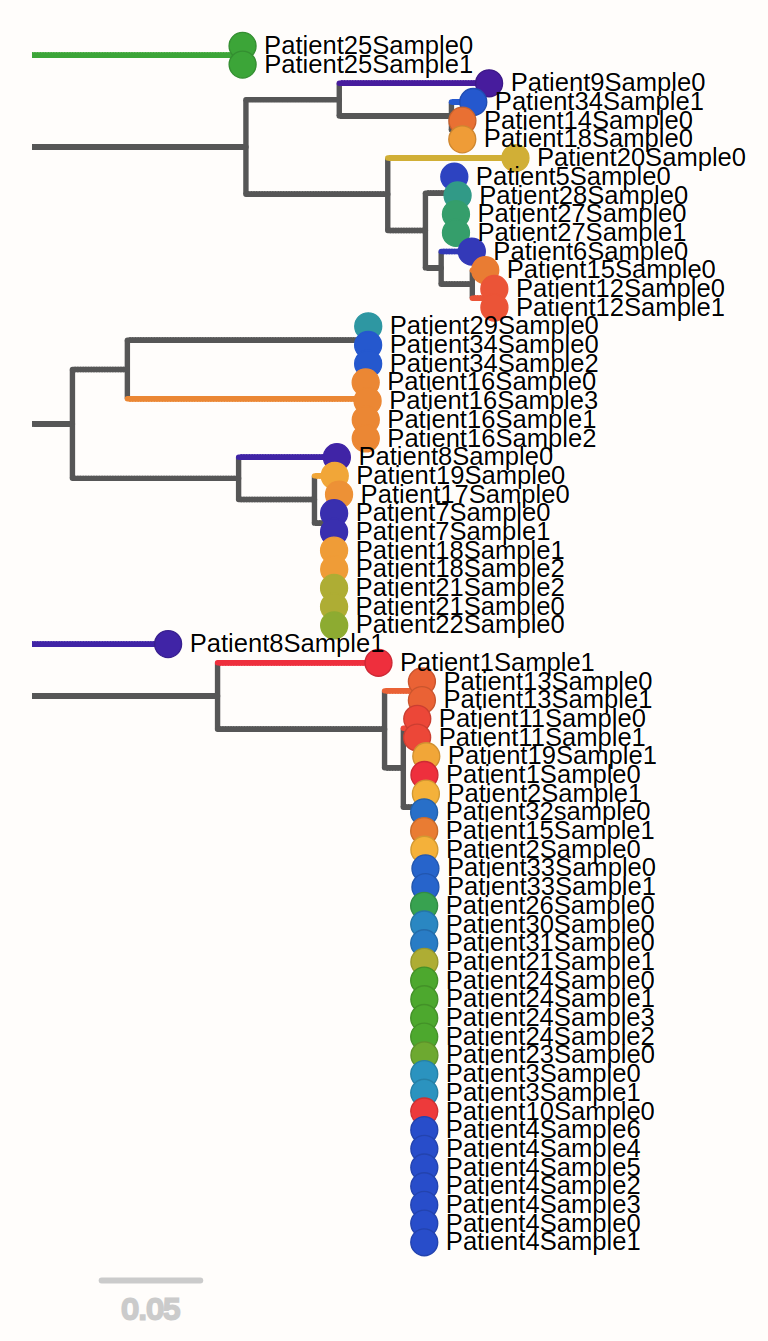
\includegraphics[scale=0.2]{181205_panXtree_overview.png}
	\caption{Phylogenic tree built for every ESBL \textit{E. coli} sample}
	\label{figure:panX}
\end{figure}


\begin{table}[]
	\begin{tabularx}{\textwidth}{|cccLL|}
		\hline
		Patient                   & Sample                   & Sample date                     & MIC cefepim {[}\textmu g/ml{]} & MIC ceftazidime {[}\textmu g/ml{]} \\ \hline
		\rowcolor[HTML]{FFCE93} 
		{\color[HTML]{000000} 12} & {\color[HTML]{000000} 0} & {\color[HTML]{000000} 09/09/14} & {\color[HTML]{000000} 4}                      & {\color[HTML]{000000} 0.75}                       \\
		& 1                        & 05/12/14                        & 12                                            & 2                                                 \\ \hline
		\rowcolor[HTML]{FFCE93} 
		16                        & 0                        & 22/06/12                        & 8                                             & 2                                                 \\
		& 1                        & 18/07/13                        & 48                                            & 8                                                 \\
		& 2                        & 01/11/13                        & 32                                            & 12                                                \\ \hline
		\rowcolor[HTML]{FFCE93} 
		24                        & 0                        & 02/05/11                        & 4                                             & 1.5                                               \\
		& 1                        & 08/15/11                        & 16                                            & 1.5                                               \\
		& 2                        & 11/28/11                        & 3                                             & 1                                                 \\ \hline
		25                        & 0                        & 15/04/11                        & 64                                            & 192                                               \\
		\rowcolor[HTML]{FFCE93} 
		& 1                        & 22/08/11                        & 6                                             & 6                                                 \\ \hline
		33                        & 0                        & 26/09/14                        & 6                                             & 6                                                 \\
		\rowcolor[HTML]{FFCE93} 
		& 1                        & 29/01/15                        & 1                                             & 1.5                                               \\ \hline
	\end{tabularx}
	\caption{Selected patients and the MIC of cefepim and ceftazidime for their ESBL \textit{E. coli} samples. Samples stained in orange were chosen as reference genomes.}
	\label{table:samples}
\end{table}
\subsection{Identification of mutations}
For patient 12,16 and 24 we chose sample 0, for patient 25 and 33 we chose sample 1 for building a reference genome. The selected samples are stained orange in \ref{table:samples}.
The output of the ONT sequencing for the reference genomes and in how many contigs they were hybrid-assembled is shown in Table \ref{table:reference_genomes} 

\begin{table}[]
	\begin{tabularx}{\textwidth}{|ccLLL|}
		\hline
		Patient & Sample & Gigabases sequneced with ONT & Hybrid-assemlied in n contigs & ONT coverage \\ \hline
		12      & 0      & 0.39                         & 6                             & 73           \\ \hline
		16      & 0      & 1.11                         & 3                             & 207          \\ \hline
		24      & 0      & 1.81                         & 17                            & 336          \\ \hline
		25      & 1      & 1.82                         & 12                            & 338          \\ \hline
		33      & 1      & 1.24                         & 6                             & 231          \\ \hline
	\end{tabularx}
	\caption{Output of ONT sequencing for the reference genomes and in how many contigs the genomes were hybrid-assemblied}
	\label{table:reference_genomes}
\end{table} 
\subsection{Identified mutations for the selected sample series}
\subsubsection{Patient 12}
Our bioinformatial pipeline revealed two mutations for patient 12 which are shown in \ref{table:patient12}. For those mutations our pipeline didn't find any annotation. 
\begin{table}[H]
	\begin{tabularx}{\linewidth}{|cccLL|}
		\hline
		\#SNP & Contig & Position & \multicolumn{2}{l|}{Nucleotide in Sample:} \\
		&        &          & 0         & \multicolumn{1}{l|}{1}    \\ \hline
		1 & 0 & 880249  & C & A \\ \hline
		2 & 0 & 4256761 & A & T \\ \hline
	\end{tabularx}
	\caption{SNPs of sample series of patient 12}
	\label{table:patient12}
\end{table} 
\subsubsection{Patient 16}
In Table \ref{table:patietn16} we show the identified mutatios for the sample series of patient 16. We identified 21 mutations, seven of those where deletions and the rest were SNPs. Our pipeline found annotation for seven mutations. Six mutations affected genes and one mutation affected a promoter. The affected genes are shown in Table \ref{table:pat16annot} and the affected promoter in Table \ref{table:pat16_prom}. This promoter annotation was obtained from the EcoCyc promoter sequences. 
\begin{table}[H]
	\begin{tabularx}{\linewidth}{|cccLLL|}
		\hline
		\#SNP & Contig & Position & \multicolumn{3}{l|}{Nucleotide in Sample:} \\
		&        &          & 0     & 1     & \multicolumn{1}{l|}{2}    \\ \hline
		1     & 0      & 109928   & C     & A     & \multicolumn{1}{l|}{C}    \\ \hline
		2     & 0      & 1895312  & A     & C     & \multicolumn{1}{l|}{A}    \\ \hline
		3     & 0      & 2101128  & G     & -     & \multicolumn{1}{l|}{-}    \\ 
		&        & 2101129  & C     & -     & \multicolumn{1}{l|}{-}    \\ 
		&        & 2101130  & A     & -     & \multicolumn{1}{l|}{-}    \\ \hline
		4     & 0      & 2375277  & C     & T     & \multicolumn{1}{l|}{C}    \\ \hline
		5     & 0      & 3797984  & A     & G     & \multicolumn{1}{l|}{A}    \\ \hline
		6     & 0      & 4200032  & T     & C     & \multicolumn{1}{l|}{T}    \\ \hline
		7     & 0      & 4353560  & G     & C     & \multicolumn{1}{l|}{G}    \\ \hline
		8     & 0      & 5112127  & G     & T     & \multicolumn{1}{l|}{G}    \\ \hline
		9     & 0      & 55597    & A     & G     & \multicolumn{1}{l|}{G}    \\ \hline
		10    & 0      & 922702   & G     & A     & \multicolumn{1}{l|}{G}    \\ \hline
		11    & 0      & 1133762  & C     & T     & \multicolumn{1}{l|}{T}    \\ \hline
		12    & 0      & 1549518  & T     & G     & \multicolumn{1}{l|}{G}    \\ \hline
		13    & 0      & 2016331  & A     & C     & \multicolumn{1}{l|}{A}    \\ \hline
		14    & 0      & 2101129  & C     & -     & \multicolumn{1}{l|}{-}    \\ 
		&        & 2101130  & A     & -     & \multicolumn{1}{l|}{-}    \\ \hline
		15    & 0      & 3920934  & A     & G     & \multicolumn{1}{l|}{A}    \\ \hline
		16    & 0      & 4333944  & C     & T     & \multicolumn{1}{l|}{T}    \\ \hline
		17    & 0      & 4459680  & C     & -     & \multicolumn{1}{l|}{C}    \\ 
		&        & 4459681  & C     & -     & \multicolumn{1}{l|}{C}    \\ \hline
		18    & 0      & 4459684  & G     & -     & \multicolumn{1}{l|}{G}    \\ 
		&        & 4459685  & A     & -     & \multicolumn{1}{l|}{A}    \\ 
		&        & 4459686  & A     & -     & \multicolumn{1}{l|}{A}    \\ 
		&        & 4459687  & G     & -     & \multicolumn{1}{l|}{G}    \\ 
		&        & 4459688  & A     & -     & \multicolumn{1}{l|}{A}    \\ 
		&        & 4459689  & G     & -     & \multicolumn{1}{l|}{G}    \\ \hline
		19    & 0      & 4459692  & A     & -     & \multicolumn{1}{l|}{A}    \\ 
		&        & 4459693  & G     & -     & \multicolumn{1}{l|}{G}    \\ \hline
		20    & 0      & 4459695  & G     & -     & \multicolumn{1}{l|}{G}    \\ \hline
		21    & 0      & 4459697  & T     & -     & \multicolumn{1}{l|}{T}    \\ \hline
	\end{tabularx}
	\caption{Mutations of the sample series of patient 16.}
	\label{table:patietn16}
\end{table}
\begin{table}[H]
	\begin{tabularx}{\linewidth}{|ccLLccc|}
		\hline
		\#SNP & Gene          & Product                                  & Type and position in gene      & \multicolumn{3}{l|}{Amino acid in Sample:} \\
		&               &                                          &                        & 0   & 1               & 2               \\ \hline
		1     & \textit{ortT} & Orphan toxin OrtT                        & Missense, 44           & P   & T               & P               \\ \hline
		2     & \textit{scrY} & Sucrose Porin                            & Missense, 104          & L   & V               & L               \\ \hline
		3     & \textit{cpdA} & Phosphodiesterase CpdA                   & In-frame deletion, 162 & L   & -   & -   \\ \hline
		4     & \textit{rpoB} & DNA-directed RNA polymerase subunit beta & Missense, 113          & V   & I               & V               \\ \hline
		5     & \textit{ftsQ} & Cell division protein FtsQ               & Missense, 207          & K   & R               & K               \\ \hline
		4     & \textit{recR} & Recombination protein RecR               & Missense, 40           & M   & T               & M               \\ \hline
		5     & \textit{hcxA} & Hydoxycarboxylate dehydrogenase A        & Missense, 332          & R   & G               & R               \\ \hline
		6     & \textit{ribA} & GRP cyclohydrolase-2                     & Missense, 68           & F   & L               & L               \\ \hline
	\end{tabularx}
	\caption{Annotation for identified Mutations, type and how they affected the peptide for patient 16.}
	\label{table:pat16annot}  
\end{table}
\begin{table}[H]
	\begin{tabular}{|lll|}
		\hline
		\#SNP & Transcription unit & Next upstream gene \\ \hline
		16    & fes-ybdZ-entF-fepE & \textit{fepA}      \\ \hline
	\end{tabular}
	\caption{Identified promoter affected by a mutation}
	\label{table:pat16_prom}
\end{table}
The mutation at position 80 in the fepA promoter is shown in the Alignment \ref{figure:alignment}. The mutation was found in the binding site of the \textsigma 70 transcription factor.  
\begin{texshade}{pat16fepa.aln}
	\showruler{1}{top}
		\feature{bottom}{1}{24..29}{fill:-}{-35}
	\feature{bottom}{1}{48..53}{fill:-}{-10}
	\feature{top}{1}{60..60}{fill:$\downarrow$}{Start of $\sigma$70 binding site}
	\hideconsensus
	\showcaption{This alignment shows the SNP in the fepA promotor. Positions marked with dashed lines are the recognition sites for $\sigma$70 factor.}
	\label{figure:alignment}
\end{texshade}
\subsubsection{Patient 24}
Identified mutations for the sample series of patient 24 are show in Table \ref{table:pat24} and the affected genes in Table \ref{table:pat24_ann}.
\begin{table}[H]
	\begin{tabularx}{\linewidth}{|cccLLL|}
		\hline
		\#SNP & Contig & Position & \multicolumn{3}{l|}{Nucleotide in Sample:} \\
			&        &          & 0     & 1     & \multicolumn{1}{l|}{2}    \\ \hline
	1     & 0      & 50032    & G            & A            & G            \\ \hline
	2     & 0      & 418564   & C            & T            & C            \\ \hline
	3     & 0      & 2048961  & A            & C            & C            \\ \hline
	4     & 0      & 2319554  & T            & A            & A            \\ \hline
	5     & 0      & 3444478  & T            & C            & T            \\ \hline
	6     & 0      & 4063226  & G            & T            & T            \\ \hline
	\end{tabularx}
	\caption{Identified mutations for patient 24}
	\label{table:pat24}
\end{table}

\begin{table}[H]
	\begin{tabularx}{\linewidth}{|ccLLccc|}
		\hline
		\#SNP & Gene          & Product                                  & Type and position in gene      & \multicolumn{3}{l|}{Amino acid in Sample:} \\
		&               &                                          &                        & 0   & 1               & 2               \\ \hline
		1     & \textit{atl}     & DNA base-flipping protein                                  & Missense, 87      & V           & M           & V           \\ \hline
		2     & \textit{imm\_2}  & Colicin-E7 immunity protein                                & Missense, 69      & K           & E           & K           \\ \hline
		3     & \textit{lldR\_2} & Lactate Dehydrogenase regulatory protein & Missense, 44      & I           & S           & S           \\ \hline
		4     & \textit{dctM\_2} & TRAP transporter large permease protein                                                        & Missense, 112     & T           & S           & S           \\ \hline
		5     & \textit{dltA}    & D-alanine--D-alanyl carrier protein ligase subunit 1           & Missense, 692     & E           & G           & E           \\ \hline
		6     & \textit{fnr}     & Fumarate and nitrate reduction regulatory protein          & Missense, 31      & C           & F & F  \\ \hline    
	\end{tabularx}
	\caption{Annotation for identified Mutations, type and how they affected the peptide for patient 24.}
	\label{table:pat24_ann}
\end{table}

\subsubsection{Patient 25}
For the sample series of patient 25 six mutations were identified, one of them is a deletion of 12 nucleotides causing a frame-shift mutation in the peptide. The mutations are shown in Table \ref{table:pat25} and their annotations in Table \ref{table:pat25_ann}.

\begin{table}[H]
	\begin{tabularx}{\linewidth}{|cccLL|}
		\hline
		\#SNP & Contig & Position & \multicolumn{2}{l|}{Nucleotide in Sample:} \\
		&        &          & 0         & \multicolumn{1}{l|}{1}    \\ \hline
	1 & 0 & 396325   & G & A \\ \hline
	2 & 0 & 396846  & G & A \\ \hline
	3 & 0 & 1996537 & - & C \\ 
	&   & 1996538 & - & C \\ 
	&   & 1996539 & - & G \\ 
	&   & 1996540 & - & T \\ 
	&   & 1996541 & - & A \\ 
	&   & 1996542 & - & C \\ 
	&   & 1996543 & - & C \\ 
	&   & 1996544 & - & A \\ 
	&   & 1996545 & - & G \\ 
	&   & 1996546 & - & C \\ 
	&   & 1996547 & - & T \\ 
	&   & 1996548 & - & G \\ \hline
	4 & 0 & 3743644 & A & G \\ \hline
	5 & 0 & 4785433 & G & A \\ \hline
	6 & 0 & 4785439 & G & A \\ \hline
	\end{tabularx}
	\caption{Identified mutations for patient 25}
	\label{table:pat25}
\end{table} 

\begin{table}[H]
	\begin{tabularx}{\linewidth}{|ccLLcc|}
		\hline
	\#SNP & Gene          & Product                                 & Type and position & \multicolumn{2}{l|}{Amino acid Sample:} \\
	&               &                                         &                   & 0                  & 1                  \\ \hline
	1     & \textit{ompR} & Transcriptional regulatory protein OmpR & Missense, 146     & R                  & H                  \\ \hline
	2     & \textit{envZ} & Osmolarity sensor protein EnvZ          & Missense, 84      & G                  & E                  \\ \hline
	3     & \textit{rfbD} & dTDP-4-dehydrorhamnose reductase        & \multicolumn{3}{l|}{Frameshift deletion, 148-295}            \\ \hline
	\end{tabularx}
	\caption{Annotation for identified Mutations, type and how they affected the peptide for patient 25.}
	\label{table:pat25_ann}
\end{table}

\subsubsection{Patient 33}
Only three mutations were found for the sample series of patient 33, they are shown in Table \ref{table:pat33} with their annotation in Table \ref{table:pat33_ann}.
\begin{table}[H]
	\begin{tabularx}{\linewidth}{|cccLL|}
		\hline
		\#SNP & Contig & Position & \multicolumn{2}{l|}{Nucleotide in Sample:} \\
		&        &          & 0         & \multicolumn{1}{l|}{1}    \\ \hline
		1 & 0 & 4008745 & A & T \\ \hline
		2 & 0 & 4675092 & T & A \\ \hline
		3 & 0 & 1996537 & A & C \\ \hline
	\end{tabularx}
	\caption{Identified mutations for patient 25}
	\label{table:pat33}
\end{table} 
\begin{table}[H]
	\begin{tabularx}{\linewidth}{|ccLLcc|}
		\hline
		\#SNP & Gene          & Product                           & Type and position & \multicolumn{2}{l|}{Amino acid Sample:} \\
		&               &                                   &                   & 0                  & 1                  \\ \hline
		1     & \textit{cydD} & ATP-binding/permease protein CydD & Missense, 368     & Q                  & L                  \\ \hline
		2     & \textit{vnfA} & Nitrogen fixation protein VnfA    & Missense, 169     & N                  & I                  \\ \hline
	\end{tabularx}
	\caption{Annotation for identified Mutations, type and how they affected the peptide for patient 16.}
	\label{table:pat33_ann}
\end{table}
\subsection{Copynumbers of ESBL genes}
Next to the reference genomes we also hybrid-assemblied and annotated the other samples of the selected sample series. This allowed us to see, if the copy numbers of ESBL genes increased while resistance evolved. Which ESBL genes where present on a plasmid or chromosomally in which sample is shown in Figure \ref{figure:esbl_genes}. For four out of five patients the copy number remained very similar. Sometimes the ESBL gene was integrated in the chromosome or an ESBL gene was replaced by a different ESBL gene. Only the sample series of patient 33 showed an increase of ESBL genes while resistance evolved. Sample 0 of patient 33 has 9 copies of CTX-M-1 while sample 1 only had one. 
\begin{figure}[H]
	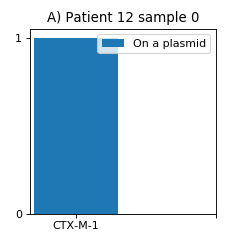
\includegraphics[width=.25\textwidth]{pat12s0.png}
	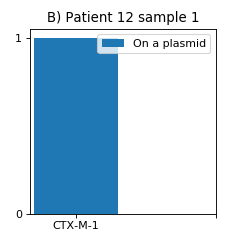
\includegraphics[width=.25\textwidth]{pat12s1.png}	
	
	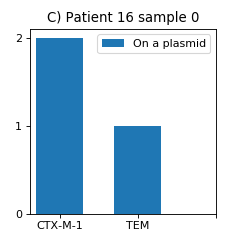
\includegraphics[width=.25\textwidth]{pat16s0.png}
	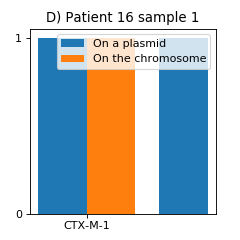
\includegraphics[width=.25\textwidth]{pat16s1.png}
	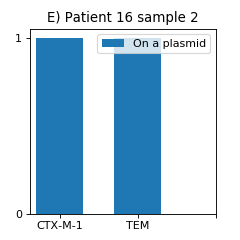
\includegraphics[width=.25\textwidth]{pat16s2.png}
	
	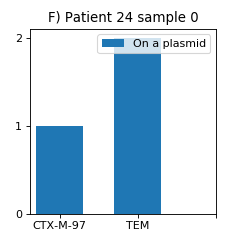
\includegraphics[width=.25\textwidth]{pat24s0.png}
	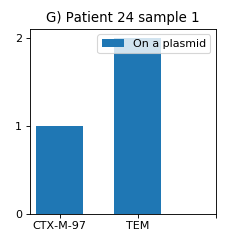
\includegraphics[width=.25\textwidth]{pat24s1.png}
	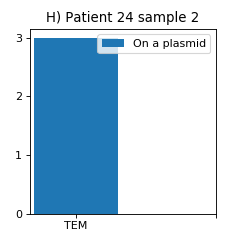
\includegraphics[width=.25\textwidth]{pat24s2.png}
	
	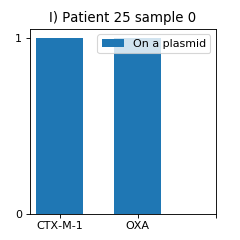
\includegraphics[width=.25\textwidth]{pat25s0.png}\hfill	
	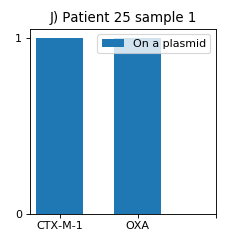
\includegraphics[width=.25\textwidth]{pat25s1.png}\hfill
	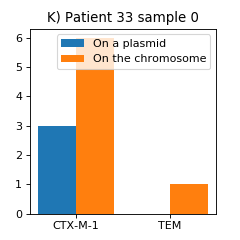
\includegraphics[width=.25\textwidth]{pat33s0.png}\hfill
	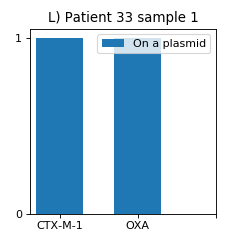
\includegraphics[width=.25\textwidth]{pat33s1.png}\hfill
	
	\caption{Copy numbers of ESBL genes. A-B: Copy numbers for patient 12 stayed the same. C-E: One CTX-M-1 was integrated in the genome for sample 1. F-H: Sample 2 lost CTX-M-97 but picked up one copy of TEM. I-J: Copy numbers for patient 25 stayed the same. K-L: Sample 1 has 8 more copies of CTX-M-1.}
	\label{figure:esbl_genes}
\end{figure}
Studying the short-reads of sample 0 mapped to the reference genome from sample 1 revealed that the coverage for sample 0 was very high for a region of 17 kilo base-pairs (kbp). This increased coverage, the genes located within this region and the GC-content is shown in Figure \ref{figure:coverage}. The gene coding for CTX-M-1 is within this 17 kbp region. This confirms that the copy number of the gene coding for CTX-M-1 is much higher in sample 0.

\begin{figure}[H]
	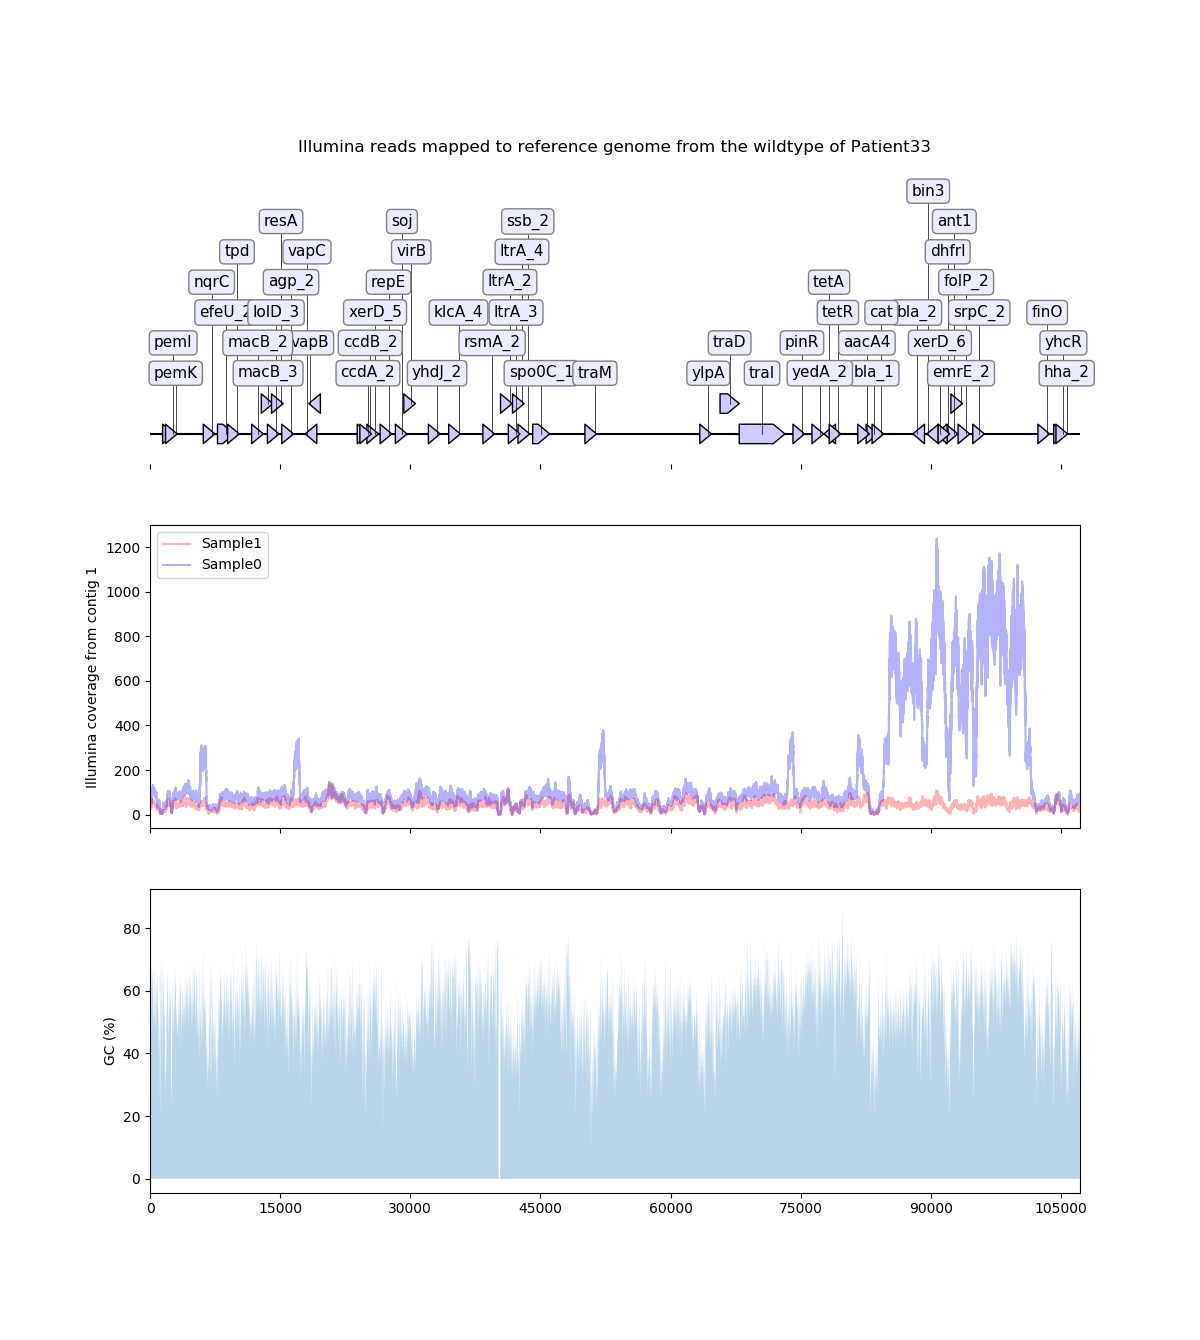
\includegraphics[scale=0.3]{coverage_pat33.png}
	\caption{Upper figure: Annotation of the whole plasmid. Middle figure: Coverage of the illumina sequencing data from sample 0 (resistant sample) and sample 1 (susceptible sample). Buttom figure: GC content.}
	\label{figure:coverage}
\end{figure}
\newpage
\newpage
\section{Morbidostat experiments}
\subsection{Contamination analysis}
\begin{table}[H]
	\begin{tabularx}{\linewidth}{|LLLLL|}
		\hline
		Stocked strain    & Total reads & Reads mapped to \textit{Bacillus cereus} & Reads mapped to \textit{E. coli} & \% of reads mapped to \textit{Bacillus cereus} \\ \hline
		pEU22\_CTX & 3810442     & 16496                                                     & 3803789                                           & 0.43                                                            \\ \hline
		pEU23\_OXA & 4329090     & 18499                                                     & 4322708                                           & 0.43                                                            \\ \hline
		pEU26\_OXA & 4040571     & 17629                                                     & 4036167                                           & 0.44                                                            \\ \hline
		K-12 MG 1655      & 4939319     & 21902                                                     & 4931214                                           & 0.44                                                            \\ \hline
	\end{tabularx}
	\caption{Illumina short-reads from every stock were mapped to a \textit{Bacillus cereus} genome from NCBI \cite{noauthor_bacillus_nodate} and the \textit{E.coli} reference genome produced with  hybrid-assembling.}
	\label{table:bacillus_reads}
\end{table}
\begin{figure}
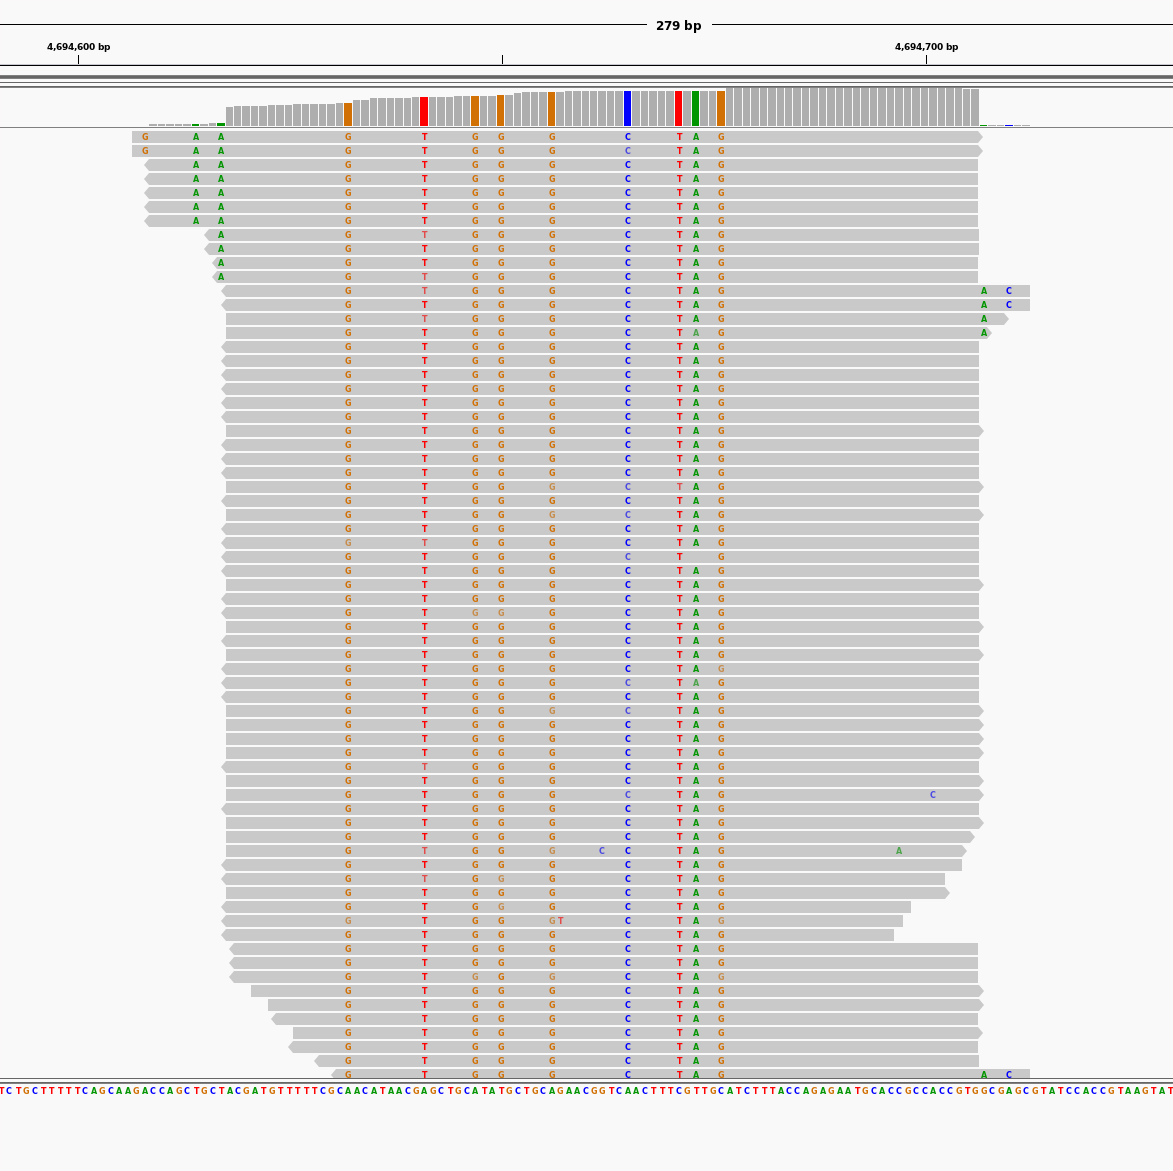
\includegraphics[width=0.8\textwidth]{bacillus_reads.png}
\caption{Alignment of short reads from pEU23\_OXA to the \textit{Bacillus cereus}. The reads map with a few SNPs which are colored. The reads also don't overlap.}
\label{figure:bacillus_reads}
\end{figure}
As visible in Table \ref{table:bacillus_reads} around 0.44 \% of all Illumina short-reads map to \textit{Bacillus cereus}. In Figure \ref{figure:bacillus_reads} one region of an alignment of the Illumina short-reads to the \textit{Bacillus cereus} genome is shown. We could see that those reads only map to very certain regions of the genome without overlapping and with a variation of a few bases. Because the reads are not overlapping and they don't map with an identity of 100 \% the stocks were not contaminated. Also the hybrid-assembly of the reference genome did not show any contigs with \textit{Bacillus cereus} sequences.
This means that around 0.44 \% of the plasmid-stocks map to conserved regions of the \textit{Bacillus cereus} genome. Therefore we expect a similar outcome for the samples from the morbidostat which were not contaminated. 

The outcome of mapping the Illumina shor-reads from the morbidostat samples to the \textit{Bacillus cereus} reference genome and the \textit{E. coli} reference genome of the sample is shown in Table \ref{table:bacillus_reads_samples}.
12 samples were not contaminated and 9 were pretty heavily contaminated.
\begin{table}[H]
	\begin{tabularx}{\linewidth}{|LccLLLL|}
		\hline
		Experiment & Vial & Sample & Total reads & Reads mapped to \textit{Bacillus cereus} & Reads mapped to \textit{E. coli} & \% of reads mapped to \textit{Bacillus cereus} \\ \hline
		01         & 1    & 1      & 6490750     & 4967611                         & 272289                  & 76.53                                \\ \hline
		01         & 2    & 1      & 7601839     & 6001106                         & 418578                  & 78.94                                \\ \hline
		01         & 3    & 1      & 2940556     & 13976                           & 2934902                 & 0.48                                 \\ \hline
		01         & 4    & 1      & 8167777     & 6150829                         & 281584                  & 75.31                                \\ \hline
		01         & 5    & 1      & 5606842     & 4089104                         & 178462                  & 72.93                                \\ \hline
		01         & 9    & 1      & 5636939     & 4466280                         & 268813                  & 79.23                                \\ \hline
		01         & 10   & 1      & 4935808     & 22368                           & 4928816                 & 0.45                                 \\ \hline
		02         & 1    & 1      & 6152378     & 26815                           & 6143228                 & 0.44                                 \\ \hline
		02         & 2    & 1      & 6926506     & 5180940                         & 291927                  & 74.80                                \\ \hline
		02         & 3    & 1      & 5142535     & 24909                           & 5136761                 & 0.48                                 \\ \hline
		02         & 3    & 2      & 6196309     & 4694898                         & 279679                  & 75.77                                \\ \hline
		02         & 4    & 1      & 4923087     & 22342                           & 4915639                 & 0.45                                 \\ \hline
		02         & 4    & 2      & 4589212     & 20628                           & 4582915                 & 0.45                                 \\ \hline
		02         & 5    & 1      & 4298753     & 17870                           & 4292083                 & 0.42                                 \\ \hline
		02         & 5    & 2      & 5189054     & 22772                           & 5181923                 & 0.44                                 \\ \hline
		02         & 7    & 1      & 5167596     & 22583                           & 5159028                 & 0.44                                 \\ \hline
		02         & 7    & 2      & 4976635     & 3015316                         & 107767                  & 60.59                                \\ \hline
		02         & 8    & 1      & 4356280     & 19067                           & 4350598                 & 0.44                                 \\ \hline
		02         & 8    & 2      & 4186125     & 18526                           & 4181356                 & 0.44                                 \\ \hline
		02         & 9    & 1      & 4182681     & 18487                           & 4176477                 & 0.44                                 \\ \hline
		02         & 10   & 1      & 3809536     & 2576863                         & 136340                  & 67.64                                \\ \hline
	\end{tabularx}
	\caption{Illumina short-reads from every morbidostat sample mapped to to a \textit{Bacillus cereus} from NCBI \cite{noauthor_bacillus_nodate} and the \textit{E.coli} reference genome produced with  hybrid-assembling.}
	\label{table:bacillus_reads_samples}
\end{table}
The identified SNPs and affected proteins are shown for every vial with samples which were not contaminated.
\subsection{Experiment 01}
\subsubsection{Vial 3}
No SNPs were found for this vial.
\subsubsection{Vial 10}
\begin{table}[H]
	\begin{tabularx}{\linewidth}{|cccLL|}
		\hline
		\#SNP & Contig & Position & \multicolumn{2}{l|}{Nucleotide in Sample:} \\
		&        &          & 0         & \multicolumn{1}{l|}{1}    \\ \hline
		1 & 0 & 3403729 & G & C \\ \hline
	\end{tabularx}
\end{table} 
\begin{table}[H]
	\begin{tabularx}{\linewidth}{|ccLLcc|}
		\hline
		\#SNP & Gene          & Product                           & Type and position & \multicolumn{2}{l|}{Amino acid Sample:} \\
		&               &                                   &                   & 0                  & 1                  \\ \hline
	1 & \textit{tomB\_1} & Hha toxicity modulator TomB & Silent, 43 & I & V \\ \hline
	
	\end{tabularx}
\end{table}
\subsection{Experiment 02}
\subsubsection{Vial 1}
No SNPs were found for this vial.
\subsubsection{Vial 3}
\begin{table}[H]
	\begin{tabularx}{\linewidth}{|cccLL|}
		\hline
		\#SNP & Contig & Position & \multicolumn{2}{l|}{Nucleotide in Sample:} \\
		&        &          & 0         & \multicolumn{1}{l|}{1}    \\ \hline
		1 & 1 & 4290 & G & T \\ \hline
	\end{tabularx}
\end{table} 
The identified SNP is affecting the cloned plasmid. More coming soon. 
\subsubsection{Vial 4}
\begin{table}[H]
	\begin{tabularx}{\linewidth}{|cccLLL|}
		\hline
		\#SNP & Contig & Position & \multicolumn{3}{l|}{Nucleotide in Sample:} \\
		&        &          & 0     & 1     & \multicolumn{1}{l|}{2}    \\ \hline
		1 & 1 & 2526   & T & T & A \\ \hline
		2 & 0 & 347328 & C & C & T \\ \hline
	\end{tabularx}
\end{table}

\begin{table}[H]
	\begin{tabularx}{\linewidth}{|ccLLccc|}
		\hline
		\#SNP & Gene          & Product                                  & Type and position in gene      & \multicolumn{3}{l|}{Amino acid in Sample:} \\
		&               &                                          &                        & 0   & 1               & 2               \\ \hline
		1 & \textit{bla}  & Beta-lactamase CTX-M-1                  & Missense, 289 & V & V & D \\ \hline
		2 & \textit{ompR} & Transcriptional regulatory protein OmpR & Nonsense, 67  & R & R & * \\ \hline
	\end{tabularx}
\end{table}
\subsubsection{Vial 5}
\begin{table}[H]
	\begin{tabularx}{\linewidth}{|cccLLL|}
		\hline
		\#SNP & Contig & Position & \multicolumn{3}{l|}{Nucleotide in Sample:} \\
		&        &          & 0     & 1     & \multicolumn{1}{l|}{2}    \\ \hline
		1 & 0 & 1570984 & C & C & T \\ \hline
		2 & 0 & 668881  & A & T & A \\ \hline
		3 & 0 & 2898640 & G & G & - \\ \hline
	\end{tabularx}
\end{table}

\begin{table}[H]
	\begin{tabularx}{\linewidth}{|ccLLccc|}
		\hline
		\#SNP & Gene          & Product                                  & Type and position in gene      & \multicolumn{3}{l|}{Amino acid in Sample:} \\
		&               &                                          &                        & 0   & 1               & 2               \\ \hline
		1 & \textit{ompC\_1} & Outer membrane protein C         & Silent, 8              & L & L & L \\ \hline
		2 & \textit{rpoD}    & RNA polymerase sigma factor RpoD & Missense, 594             & L & Q & L \\ \hline
		3 & \textit{ompF}    & Outer membrane protein F         & Frameshift, 319 & G & G & A \\ \hline
	\end{tabularx}
\end{table}
\subsubsection{Vial 8}
No SNPs were found for this vial.
\subsubsection{Vial 9}
\begin{table}[H]
	\begin{tabularx}{\linewidth}{|cccLL|}
		\hline
		\#SNP & Contig & Position & \multicolumn{2}{l|}{Nucleotide in Sample:} \\
		&        &          & 0         & \multicolumn{1}{l|}{1}    \\ \hline
		1 & 0 & 3076603 & A & T \\ \hline
	\end{tabularx}
\end{table} 
\begin{table}[H]
	\begin{tabularx}{\linewidth}{|ccLLcc|}
		\hline
		\#SNP & Gene          & Product                           & Type and position & \multicolumn{2}{l|}{Amino acid Sample:} \\
		&               &                                   &                   & 0                  & 1                  \\ \hline
1 & \textit{iscR} & HTH-type transcriptional regulator IscR & Missense, 56 & C & S \\ \hline

		
	\end{tabularx}
\end{table}
